\documentclass[a4paper,12pt]{article}
\usepackage[section] {placeins}
\usepackage{morefloats}
%\usepackage{achemso}
\usepackage{graphicx}
\usepackage{epstopdf}
\usepackage{bbm}
\usepackage{textcomp}
\usepackage{amsfonts}
\usepackage{amssymb}
\usepackage{amsthm,amsmath,amssymb,amstext}
\usepackage{booktabs}
\usepackage{float}
\usepackage{mathrsfs}
\usepackage{pgf}
\usepackage{subfigure}
\usepackage{setspace}
\usepackage{makecell}
\usepackage{url}
\usepackage[top=3cm,left=1.5cm,right=1.5cm,bottom=2cm,foot=1cm]{geometry}
\usepackage[resetlabels,labeled]{multibib}
\renewcommand{\labelenumi}{(\roman{enumi})}
\usepackage{multirow}
\usepackage{isomath}
\usepackage{mathtools}
\usepackage{hyperref}
\renewcommand{\thefigure}{S\arabic{figure}}
\renewcommand{\thetable}{S\arabic{table}}
\newcommand{\mvec}[1]{\vectorsym{#1}}
\newcommand{\mmat}[1]{\matrixsym{#1}}
\newcommand{\icol}[1]{% inline column vector
  \begin{bsmallmatrix}#1\end{bsmallmatrix}^\intercal%
}
\newcommand{\irow}[1]{% inline column vector
 \begin{bsmallmatrix}#1\end{bsmallmatrix}%
}
\usepackage[final]{changes} 
    \definechangesauthor[name={Zhu},color=red]{Z.}
\newcommand{\mcol}[1]{{\color{blue}#1}}
\makeatletter
\newcommand\sixteen{\@setfontsize\sixteen{17pt}{6}}
\renewcommand{\maketitle}{\bgroup\setlength{\parindent}{0pt}
\begin{flushleft}
\sixteen\bfseries \@title
\medskip
\end{flushleft}
\textit{\@author}
\egroup}
\makeatother

\doublespacing
\title{Roles of Physicochemical and Structural Properties of RNA Binding Proteins in Predicting the Activities of Trans-Acting Splicing Factors with Machine Learning}

\author{\textbf{Lin~Zhu}$^{1}$ \textbf{and} \textbf{Wenjin Li}$^{1,*}$\\ \medskip
$^{1}$ Institute for Advanced Study, Shenzhen University, Shenzhen 518060, China\\
\textbf{*Correspondence:}\\
Wenjin Li, Room 720, Institute for Advanced Study, Shenzhen University, Shenzhen 518060, China; E-mail: liwenjin@szu.edu.cn; Tel: +86-0755-26942336}


\begin{document}
\maketitle
\section*{Supplementary materials}
Table S1: The performance of 647 features with the number of component ranging from 1 to 10.

\noindent
Table S2: mRMR features list.

\noindent
Table S3: The Spearman\added{'s correlation} coefficient of the mRMR features list.

\noindent
Table S4: \replaced{F}{The f}orward feature list.

\noindent
Table S5: Spearman\added{'s correlation} coefficient of the forward features list.

\noindent
Table S6: \replaced{P}{The p}erformance of Wang's features with the number of components ranging from 1 to 10.

\noindent
Table S7: \replaced{O}{The o}riginal dataset consists of 85 splicing factors.

\noindent
Table S8: \added{Conversion of }85 experimentally tested splicing factors into a 700-dimensional feature matrix by feature encoding.

\noindent
Table S9: \added{Construction of }a 647-dimensional feature matrix\deleted{was constructed} from the 700-dimension feature matrix by removing the features that are almost 0 in all samples.

\begin{figure}
\centering
\includegraphics[width=0.9\textwidth]{Figure S1:mRMR_all_matrics.png}
\caption{\label{pic1} Curves of five metrics produced by the mRMR features. Three metrics $R^2$, Pearson's coefficient and Spearman's coefficient show a similar uptrend, and $RMSE$ and $NRMSE$ display a similar downtrend.  }
\end{figure}

\begin{figure}
\centering
\includegraphics[width=0.9\textwidth]{Figure S2:forward_all_metrics.png}
\caption{\label{pic2} Curves of five metrics produced by using the forward feature searching strategy. \replaced{T}{As can be seen from this figure: t}hree metrics $R^2$, Pearson's coefficient and Spearman's coefficient show a similar trend, and $RMSE$ and $NRMSE$ display a similar trend. }
\end{figure}

\begin{figure}
\centering
\includegraphics[width=0.9\textwidth]{Figure S3:PLS-93.png}
\caption{\label{pic3} \replaced{F}{It is a f}itting graph produced by 93 features, showing the best feature subset (93 features) with good performance. }
\end{figure}

\begin{figure}
\centering
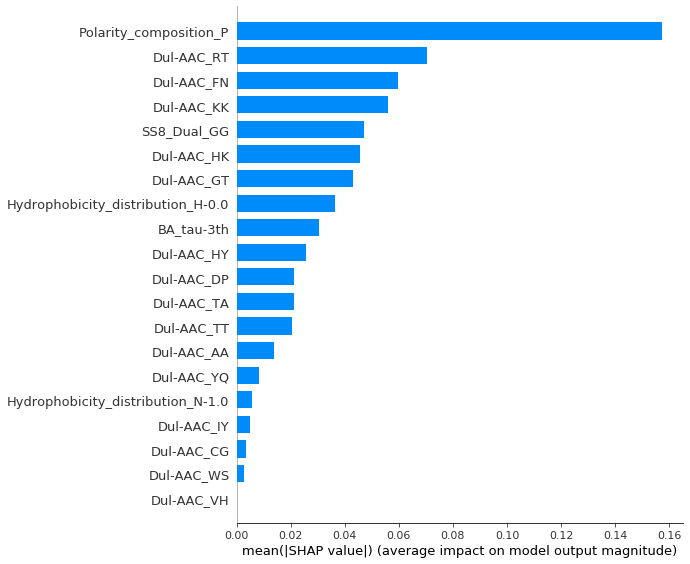
\includegraphics[width=0.9\textwidth]{shap_85_barpng.png}
\caption{\label{pic4} SHAP plot based on 5-fold cross-validation. We calculated the shap\_values for every model and its corresponding 17 validation RBPs, merged 5 shap\_values into one explainer, and visualized this explainer using SHAP bar plot.}
\end{figure}

\begin{figure}
\centering
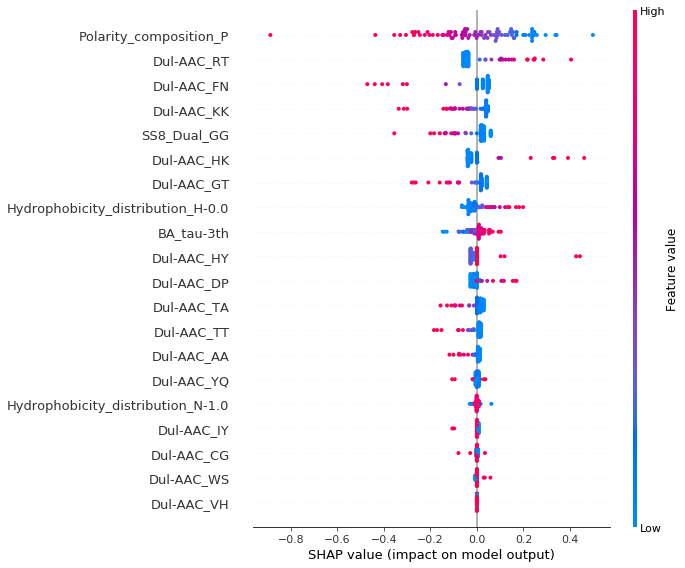
\includegraphics[width=0.9\textwidth]{shap_85.png}
\caption{\label{pic5} SHAP plot based on 5-fold cross-validation. We calculated the shap\_values for every model and its corresponding 17 validation RBPs, merged 5 shap\_values into one explainer, and visualized this explainer using SHAP beeswarm plot}
\end{figure}
\end{document}